\chapter{Chaotic dynamics in differential equations}
\section{Introduction to chaos theory and one example}

For the autonomous vector field in $\mathbb{R}^{2}$ the phase portrait and movement is fully determined; this is described in Section \ref{2.4}. But when the phase space is not so simple, interesting phenomena can happen.

\begin{figure}[!ht]
	\centering
	
\includegraphics [scale=1.5]{jtr51}
	\caption{Transitivity and mixing.}
	\label{fig:5.1}
\end{figure}

For example, a fixed vector field
$$
\dot{\varphi}_{1}=\omega _{1},\dot{\varphi}_{2}=\omega _{2}
$$
on the torus $\mathbb{T}^{2}=\left\{ \left( \varphi _{1}, \varphi_{2}\right) \right\} $ can have dense phase curves, i.e. when $omega_{2}/\omega _{1}$ is irrational. Then the phase curves are dense (as in Figure \ref{fig:4.1} above) and the motion is \emph{quasi-periodic}, which means that the solution returns roughly periodically to each small area of the phase space. In addition, you can reach any other small area from any small area. Such property is called \emph{transitivity} in the theory of Dynamic Systems. The movement is not fully deterministic, because after a long time it is difficult to say where the evolving particle is. However, this is not a chaotic movement, because if at the beginning we had a focused area of the phase space, then this area retains its focused shape during evolution. Meanwhile, in a \emph{chaotic movement}, such a cell begins to `dissolve' in the phase space.

\begin{example} (Transitivity and chaos).
	A good example of a situation illustrating the difference between transitivity and chaos are two glasses of water, such that one dropped in a small drop of oil and the other one poured the same amount of juice (Figure \ref{fig:5.1}). The oil droplet will drift, visit every spot in the water, and the juice will start to dissolve, filling the entire water area evenly (this property is also called \emph{mixing}).
\end{example}

\begin{figure}[!ht]
	\centering
	
\includegraphics [scale=1.5]{jtr52}
	\caption{Swing.}
	\label{fig:5.2}
\end{figure}

Perhaps the simplest differential systems in which chaos can be observed are periodic non-autonomous systems of the form
\begin{equation}
\label{5.1}
\dot{x}=v(t,x),\text{ \ \ }x\in M,\text{ \ \ }v(t+T,x)=v(t,x),
\end{equation}
where $M$ is a $2-$dimensional variety. As we know, such a system can be treated as autonomous in the expanded phase space $\mathbb{S}^{1}\times M$. Then it is convenient to work with the monodromy map (after the period)
$$
\mathcal{P}:M\longmapsto M,\text{ \ \ \ } \mathcal{P}=g_{0}^{T},
$$
where $g_{s}^{t} = \phi(t; x_0, s)$, $\phi(s;x_0, s) = x_0$, is a $2-$parameter family of diffeomorphisms defining evolution. In terms of the extended phase space it is the conversion of the return map to the hypersurface $\left\{0\right\} \times M$. In the monograph of J. Guckenheimer and P. Holmes \cite{GuHo}, an example of the Duffing system is analyzed with the external force
$$
\ddot{x}=x-x^{3}+\varepsilon \left\{ \cos (\omega t)-ax\right\} .
$$
We will take a slightly different example.

\begin{example}(Swing).
	Let be the equation
	$$
	\ddot{x}=-\sin x+\varepsilon \cos (\omega t),\
	$$
	where $\varepsilon \cos \left( \omega t\right) $ is a small periodic external force, with the period $T=2\pi /\omega $. This can be interpreted as the equation of a swing with a girl, which performs periodic crouching (see Figure \ref{fig:5.2}). You can also treat this system as a subsystem of the $4-$dimensional autonomous system
	$$
	\dot{x}=y,\text{ \ }\dot{y}=-\sin x+\varepsilon z,\text{ \ }\dot{z}=\omega u, \text{ \ }\dot{u}=-\omega z.
	$$
	
	However, let's focus on the expanded phase space $\mathbb{S}^{1}\times M$, where $M=\mathbb{S}^{1}\times \mathbb{R}$ is a cylinder and we have
	\begin{equation}
	\label{5.2}
	\dot{t}=1,\text{ \ \ \ }\dot{x}=y,\text{ \ \ }\dot{y}=-\sin x+\varepsilon
	\cos (\omega t).
	\end{equation}
	For a non-perturbed situation ($\varepsilon =0$), the phase portrait is known (see Figure \ref{fig:2.1} above); we present it in Figure \ref{fig:5.3}, where the upper and lower edges of the cylinder are shown as concentric dotted circles. We are interested in what will happen with the separatrix loop $\Gamma$ of the saddle point $x=\pi$, $y=0$.
	
	\begin{figure}[!ht]
		\centering
		
\includegraphics [scale=1.4]{jtr53}
		\caption{Phase portrait for a pendulum.}
		\label{fig:5.3}
	\end{figure}
	
	\begin{figure}[!ht]
		\centering
		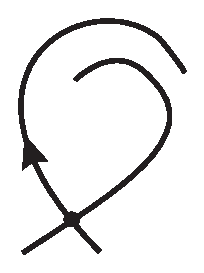
\includegraphics [scale=1.4]{jtr54}
		\caption{Separation of the saddle separatrices for the vector field.}
		\label{fig:5.4}
	\end{figure}
	
	If the perturbation was independent of time, then the expected phase portrait of the disturbed field would be as in Figure \ref{fig:5.4}, that is, the separatrices of the saddle point would be separated. However, in the case of a non-autonomous system, but periodically due to time, the phase portrait of a non-perturbed system should be treated as the dynamics of the transformation of monodromy. In the perturbed system, separatrices are not obliged to disconnect. We expect them to cross transversally, as in Figure \ref{fig:5.5}. We'll show it below.
	\begin{figure}[!ht]
		\centering
		
\includegraphics [scale=1.4]{jtr55}
		\caption{Disconnection of saddle separatrices for diffeomorphism.}
		\label{fig:5.5}
	\end{figure}
	
	The solution of the non-perturbed system, corresponding to the upper separatrix loop, is the following
	\begin{equation}
	\label{5.3}
	x=x_{0}(t)=\pi -4\tan ^{-1}e^{-(t-t_{0})},\text{ \ }y=y_{0}(t)=2/\cosh
	(t-t_{0})
	\end{equation}
	(compare Task 2.44). It has the property that $x(t_{0})=0$, $y(t_{0})=2$ and the value of the first integral
	\begin{equation}
	\label{5.4}
	H(x,y)=\frac{1}{2}y^{2}-\cos x
	\end{equation}
	at those points is $1$ (see Figure \ref{fig:5.6}).
	\begin{figure}[!ht]
		\centering
		
\includegraphics [scale=1.4]{jtr56}
		\caption{Determination of the Mielnikov integral.}
		\label{fig:5.6}
	\end{figure}
	
	For the study of the perturbed system ($\varepsilon \not=0$) we will use the whole family of monodromy transformations
	$$
	\mathcal{P}_{z}=g_{z}^{z+T}:M\longmapsto M,\text{ \ \ \ }z\in \lbrack 0,T],
	$$
	where $M=\mathbb{S}^{1}\times R$ is identified with a cut $\left\{ z\right\} \times M$ in the expanded phase space $\left(\mathbb{R} /T\mathbb{Z}\right) \times M$. Each transformation $\mathcal{P}_{z}$ has its fixed point $q(z)$ (identified with $p(z) = q(z) + (2\pi, 0)$); this point depends on $z$ and $\varepsilon$ and lies close to the point $x=-\pi$, $y=0$. Because it is a fixed and hyperbolic point (saddle), it has its stable submanifold $W^{s}(p(z))$ and unstable $W^{u}(q(z))$ (see Figure \ref{fig:5.6}); of course, these submanifolds also depend on $z$ and $\varepsilon$.
	
	Select the cut $S=\left\{ x=0,1<y<3\right\} $ transversal to $W^{s}(p(z))$ and to $W^{u}(q(z))$. Let $\phi (t)$ (respectively $\psi (t)$) be a solution with the initial condition $\phi (z)=S\cap
	W^{s}(p(z))$ (respectively $\psi (z)=S\cap W^{u}(q(z))))$. Of course, $\phi (t)\rightarrow p(z)$ at $t\rightarrow +\infty $ and $\psi
	(t)\rightarrow q(z)$ at $t\rightarrow -\infty$. In addition, $\mathcal{P}%
	_{z}(\phi (z))=\phi (z+T)$ and $\mathcal{P}_{z} (\psi (z)) = \psi (z+T)$ (invariance of the submanifold).	
	
	The intersection of the stable and unstable submanifolds is the situation when $\phi (z)=\psi (z)$ for the corresponding $z$. As in the case of perturbations of the autonomous Hamiltonian systems (see Example \ref{example:4.5}), the distance between $\phi (z)$ and $\psi (z)$ is calculated using the difference of the value of the first integral at these points,
	$$
	\Delta H|_{S}=H(\psi (z))-H(\phi (z))=\left[ H(\psi (z))-H(q(z))\right]
	+\left[ H(p(z))-H(\phi (z))\right] .
	$$
	We have
	$$
	\begin{array}{lll}
	H(\psi (z))-H(q(z)) &=&\int_{-\infty }^{z}\dot{H}dt=\varepsilon \int_{-\infty
	}^{z}y\cos \left( \omega t\right) dt, \\
	H(p(z))-H(\phi (z)) &=&\int_{z}^{\infty }\dot{H}dt=\varepsilon
	\int_{z}^{\infty }y\cos \left( \omega t\right) dt.
	\end{array}
	$$
	Therefore, $\Delta H=\varepsilon \int_{-\infty }^{\infty } y\cos \left( \omega t\right) dt$, which we shall approximate by putting $y=y_{0}(t)$ from formula \eqref{5.3}. We get the so-called \textbf{Mielnikov integral} (analog of Abel integral)
	\begin{equation}
	\label{5.5}
	\Delta H=\varepsilon M(z)+O(\varepsilon ^{2})=\varepsilon \cdot
	2\int_{-\infty }^{\infty }\frac{\cos \omega t}{\cosh (t-z)}dt+O(\varepsilon
	^{2}).
	\end{equation}
\end{example}

It is not difficult to show the following
\begin{lemma}\label{lemma:5.3}
	If $M\left( z_{0}\right) =0$ and $M^{\prime }(z_{0})\not=0$, then the submanifolds $W^{s}(p(z))$ and $W^{u}(q(z))$ transversally at a point close to $S$ \emph{(Task 5.5)}.
\end{lemma}

It turns out that the Mielnikov integral from the formula \eqref{5.5} is countable. Substituting $s=e^{-t}$ (with $ds=-sdt$) we get
$$
M(z)=-2\int_{0}^{\infty }\frac{e^{i\omega z}s^{-i \omega}+e^{-i\omega z}s^{i\omega }}{1+s^{2}}ds.
$$
\begin{figure}[!ht]
	\centering
	
\includegraphics [scale=2]{jtr57}
	\caption{Contour of integration.}
	\label{fig:5.7}
\end{figure}

We calculate the integral $I=\int_{0}^{\infty} s^{i\alpha} (1+s^{2})^{-1}ds$ by the contour method. The integral along the contour from Figure \ref{fig:5.7}, in the boundary with the radius of circles going to $0$ and $\infty $ respectively, is
$$
\begin{array}{lll}
(1-e^{-2\pi i\alpha })I &=&2\pi i\left\{ \textrm{res}_{s=i}s^{i\alpha
}(1+s^{2})^{-1}+\textrm{res}_{s=-i}s^{i\alpha }(1+s^{2})^{-1}\right\} \\
&=&\frac{2\pi i}{2i}\left( e^{-\pi \alpha /2}-e^{-3\pi \alpha /2}\right) = 2\pi e^{-\pi \alpha }\sinh \left( \pi \alpha /2\right).
\end{array}
$$
That gives $I=\pi /(2\cosh (\pi \alpha /2))$ and
$$
M(z)=-2\pi \frac{\cos (\omega z)}{\cosh (\pi \omega/2)}.
$$

It is easy to see that this function satisfies the requirement $M^{\prime}|_{M=0} \not = 0$.

We have found at least one point $r_{0}$ of intersection of the stable and unstable manifolds fixed point $q=q(0)$ for the diffeomorphism
$$
\mathcal{P}=\mathcal{P}_{0}:U\longmapsto U,
$$
where $U$ is a certain environment of the separatrix loop $\Gamma$ of the saddle $x=\pm \pi$, $y=0$, and $\mathcal{P}_{0}$ is a distinguished transformation of monodromy from the native $\left\{ \mathcal{P}_{z} \right\} $ (with hyperbolic fixed points $q(z)$). But there are many more such points; they are of the form $r_{n} = \mathcal{P}^{n}(r_{0})$,  $n\in \mathbb{Z}$. At $n\to \infty $ and $n\to \infty $ the points $r_{n}$ strive to the fixed point $q_{0}$.

However, the submanifolds $W^{s}=W^{s}(q(0))$ and $W^{u}=W^{u}(q(0))$ behave at least as non-standard. For example, the variety $W^{u}$ in going through more and more points $r_{n}$ ($n\to \infty$) begins to become more and more parallel to itself, but in the vicinity of the saddle $q$ (i.e. to the local unstable variety $W_{loc}^{u}$). Of course, between the points $r_{n}$ and $r_{n+1}$, it makes a sharp turn. The same is more or less the case with the variety of $W^{s}$ when passing through the points $r_{n}$ for $n\to  -\infty $ and between these points. In particular, the $W^{u}$a nd $W^{s}$, highlighted above, begin to intersect in other points (than $r_{n}$).Until they start to think about what is happening at further iterations; for example, pieces of $W_{u}$ in parallel to $W_{loc}^{u}$ become longer and longer (see Figure \ref{fig:5.8}).
\begin{figure}[!ht]
	\centering
	
\includegraphics [scale=1.4]{jtr58}
	\caption{Intersection of a stable submanifold with an unstable submanifold.}
	\label{fig:5.8}
\end{figure}

\subsection*{Tasks}
\begin{task}
	Show that if $g_{s}^{t}$ is a $2-$parameter family of diffeomorphisms defining the evolution of a non-autonomous vector field $\dot{x}=v(t,x)$, which is periodic with a period $T$ respect to time, then $g_{s+T}^{t+T}=g_{s}^{t}$.
\end{task}

\begin{task}
	Prove Lemma \ref{lemma:5.3}.
	
	Indication: First, show that (as close to the phase curve from equation \eqref{5.3}) in the neighborhood of the point $x = 0$, $y = 1$ submanifolds $W^{s}(p(z))$ and $W^{u}(q(z))$ are lying horizontally, i.e. are graphs of some functions from $x$. For $z = z_0$ we will treat them as graphs of the functions $F$ and $G$ from a certain segment $J$ (on the $x-$axis) to the cut $S$, where $S$ is parameterized by $H|_{S}$.
	
	Second, the transformations $\mathcal{P}_{z_{0}}$ and $\mathcal{P}_{z}$ are coupled, $\mathcal{P}_{z} = g_{z_{0}}^{z}\circ \mathcal{P}_{z_{0}} \circ \left( g_{z_{0}}^{z}\right) ^{-1}$. Infer from here that $W^{s}(p(z))=g_{z_{0}}^{z}(W^{s}(p(z)))$ and the same with $W^{u}$. The transformations $g_{z_{0}}^{z}$ are close to the transformations $g_{0}^{z-z_{0}}|_{\varepsilon =0}$ of the phase stream of the unperturbed system \eqref{5.2}, which in the neighborhood of the point $x = 0$, $y = 2$ is roughly `clockwise'. Hence, it follows that when the variety $z$ is changed $W^{s}(p(z))$ arise from the variety $W^{s}(p(z_{0}))$ by `moving' it. Thus it follows that if $x_{0}(t)$ is set as in \eqref{5.3}, the function $H=F(x)$, whose graph is $W^{s}(p(z_{0}))$, can be set to a first approximation as
	$$
	F(x)\approx H\circ \phi \left( x_{_{0}}^{-1}(x)\right) .
	$$
	Similarly, the graph of the $G(x) \approx H \circ \psi \left( x_{0}^{-1} (x)\right)$ function first deals with $W^{u}(q(z_{0}))$. The difference $G(x)-F(x)\approx \Delta H\approx \varepsilon M(z)$ show that the transversality condition $W^{s}$ and $W^{u}$ results from the property: $\frac{d}{dx}\left( G-F\right) \not=0$ for $G-F=0$.
\end{task}


\section{The Smale horseshoe map, Anosov diffeomorphisms and attractors}

Probably S. Smale was the first who understood the phenomenon from the end of the previous chapter and described it in strict mathematical terms. In Figure \ref{fig:5.9} we see a (slightly curvilinear) `rectangle' $R$ along the local stable variety $W_{loc}^{s}$ which, under the action of the correspondingly high iteration of the transformation $\mathcal{P}$, passes to a figure that cuts $R$ in two places. One can choose the parameters defining the rectangle $R$ so that it actually takes place (we do not do this, but we can refer the reader back to R. Devaney's books \cite{Dev}, C. Robinson \cite{Rob} and W. Szlenek \cite{Szl}).

\begin{figure}[!ht]
	\centering
	
\includegraphics [scale=1.4]{jtr59}
	\caption{Generating horseshoe transformation.}
	\label{fig:5.9}
\end{figure}

A model example of the transformation as in Figure \ref{fig:5.9} is the transformation of Smale horseshoe shown in Figure \ref{fig:5.10}.

\begin{definition} (Smale horseshoe).
	We have an (authentic) rectangle $A$ on the plane with which we perform the following operations. First, extend it in the vertical direction and narrow it in the horizontal direction. Next, we bend our elongated rectangle and place it on the plane so that it intersects the output rectangle along two parallel vertical stripes
	$$
	f(A)\cap A=A_{1}\cup A_{2}.
	$$
	In this way, we get a new figure, designated $f(A)$, where $f:A\longmapsto f(A)$ is a \textbf{horseshoe diffeomorphism}.\footnote{You can extend this transformation. Let's stick  a semicircle to the bottom and top bases of $A$ and mark the new figure by $M$. Let us extend $f$ onto the semicircle so that their images adhere to the lower ends $f(A)$. Assuming that the new figure lies completely in $M$, we get a well-defined diffeomorphism $f:M\longmapsto M$.}
\end{definition}

Smale horseshoe, although simply defined, is not so simple at all. It is easy to say that $f^{2}(A)\cap A$ consists of 4 vertical bars; more generally, $f^{n}(A)\cap A$ consists of $2^{n}$ horizontal stripes (Task 5.14). On the other hand, $f^{-1}(A)\cap A=f^{-1}(A\cap f(A))$ consists of two horizontal stripes; more generally, $f^{-m}(A)\cap A$, $n>0$, consists of $2^{m}$ horizontal and thin stripes (Task 5.15). Thus $f^{n}(A)\cap f^{-m}(A)$, $m,n>0$, consists of $2^{n}\times 2^{m}$ small rectangles. Very important is the following set
\begin{equation}
\label{5.6}
\Lambda =\bigcap_{n\in \mathbb{Z}}f^{n}(A).
\end{equation}

\begin{figure}[!ht]
	\centering
	
\includegraphics [scale=1.4]{jtr510}
	\caption{Smale horseshoe.}
	\label{fig:5.10}
\end{figure}

It is easy to check that it is a set invariant to $f:$\ $f(\Lambda )=f^{-1}(\Lambda )=\Lambda $ (Task 5.16). We can say more about $\Lambda $ and about $f|_{\Lambda}$, but first we should introduce one definition.

\begin{definition}
	Let $\Sigma =\Sigma _{k}=\left\{ 1,\ldots ,k\right\} ^{\mathbb{Z}}$ be a numerable Cartesian product of a fixed $k-$elements set; it consists of strings $a=\left( \ldots ,a_{-1},a_{0},a_{1},\ldots \right)$, $a_{j}\in \left\{
	1,\ldots ,k\right\}$. We define the transformation $\sigma :\Sigma \longmapsto \Sigma $ as follows:
	$$
	\sigma \left(a _{j}\right)=a_{j+1}.
	$$
	The dynamic system $\left( \Sigma ,\sigma \right) $ defined above is called a \textbf{symbolic system}, or a \emph{shift map}.
	
	On the space $\Sigma$ the product topology is introduced, where the surroundings of the given symbol sequence $a=\left( \ldots, a_{-1}, a_{0}, a_{1}, \ldots \right) $ are \emph{cylindrical sets} of the form
	$$
	\left\{ b=\left( \ldots ,b_{-1},b_{0},b_{1},\ldots \right)
	:b_{-M}=a_{-M},b_{-M+1}=a_{-M+1},\ldots ,b_{N}=a_{N}\right\}
	$$
	(for fixed $ M, N $). $\Sigma$ is also a metric space, because the distance of two strings is $\textrm{dist}\left(a, b\right) = \sum_{n \in Z}2^{ -\left\vert n\right\vert }\left\vert a_{n} - b_{n} \right\vert$.
\end{definition}

It takes place the following

\begin{theorem}
	There is a homeomorphism $\Phi: \Lambda \longmapsto \Sigma _{2}$, which conjugates $\sigma $ with $f|_{\Lambda }:$
	$$
	\sigma \circ \Phi =\Phi \circ f.
	$$
	\begin{proof}
		Transformation $\Phi $ is easy to define. If $x\in \Lambda $, we put $\Phi (x)=\left(
		\ldots ,a_{-1},a_{0},a_{1},\ldots \right)$, where
		$$
		a_{n}=1\text{ \ if \ }f^{n}(x)\in A_{1}\text{ \ and \ }a_{n}=2\text{ \ if \ } f^{n}(x)\in A_{2}.
		$$
		The conjugation property works directly (Task 5.18). Therefore, it remains only to check the continuity and reversibility of the transformation $\Phi$.
		
		These two properties result from hyperbolic transformation of the horseshoe: in the horizontal direction is compression with the constant $\lambda _{1}<1$ and in the vertical direction we have tension with the constant $\lambda _{2}>1$. Thus, rectangles, appearing at the location of points $x$, i.e., \begin{equation}
		\label{5.7}
		\left\{ x:f^{-M}(x)\in A_{a_{-M}},\ldots ,f^{N}(x)\in A_{a_{N}}\right\} ,
		\end{equation}
		become exponentially small with $M$ and $N$ very large. We only get one point in the border (reversibility). Small sizes of sets \eqref{5.7} correspond to the small cylindrical sets in $\Sigma_2$; this is exactly the continuity of $\Phi$ and $\Phi ^{-1}$.
	\end{proof}
\end{theorem}

Since $\Lambda $ is the only invariant set in rectangle $A$, all the interesting dynamics of the transformation of the horseshoe are limited to the dynamics of $f|_{\Lambda }$. Thanks to the above theorem, it is the same dynamics as for the symbolic transformation of $\sigma $ on $\Sigma$. On the other hand, the symbolic transformation is pleasant to study. It has the following interesting properties.

\begin{proposition}
	The periodic points of $\sigma $ are dense in the symbolic space $\Sigma $.
	\begin{proof}
		Let $a=\left( \ldots, a_{p-1}, a_{0},\ldots, a_{p-1}, a_{0}, a_{1}, \ldots, a_{p-1}, a_{0}, \ldots\right) \in \Sigma $. For a large $N> 0$ all sequences $b=\left(\ldots ,b_{-1},b_{0},b_{1},\ldots \right) $ such that $b_{-N}=a_{-N},\ldots ,b_{N}=a_{N}$ are close to $a$. Thus, the sequence formed from the block $\left( a_{-N},\ldots ,a_{N}\right) $ (length $2N + 1$) and periodically repeated is also close. It corresponds to the periodic point of $\sigma$ of period $2N + 1$.
	\end{proof}
\end{proposition}

\begin{proposition}
	The dynamic system $\left( \Sigma, \sigma \right) $ is transitive, i.e. for any open subsets $U,V\subset \Sigma $ there exists $n>0$ such that $f^{n}(U)\cap V\not=\varnothing.$
	\begin{proof}
		It suffices to consider the case when $U$ and $V$ are cylindrical sets defined by means of blocks $\left(
		a_{1},\ldots ,a_{M}\right) $ and $\left( b_{1},\ldots ,b_{N}\right)$. Then just take any sequence with the block $\left( a_{1},\ldots, a_{M},b_{1},\ldots b_{N}\right) $ (length $M + N$).
	\end{proof}
\end{proposition}

\begin{remark}
	One can introduce on $\Sigma$ the probabilistic product measure $\mu$, such that $\mu \left( \left\{ a_{0}=j\right\} \right) =1/k$ (Bernoulli measure). It turns out to be invariant to the $\sigma$ shift. In addition, there is a mixing property that was mentioned at the beginning of the chapter and which do not want to strictly define. Therefore, the Smale horseshoe system as well as the swing system are chaotic systems.
\end{remark}

The subset $\Lambda \subset \mathbb{R}^{2}$, invariant for transforming the Smale horseshoe, has one more important property. Namely, it is \textbf{hyperbolic}, which means that induced linear transformations $f_{\ast }(x):T_{x}\mathbb{R}^{2}\longmapsto
T_{f(x)}\mathbb{R}^{2}$ are hyperbolic (they have one eigenvalue $\lambda _{1}\in \left( 0,1\right) $ and a second $\lambda _{2}>1$).

Unfortunately, the set $\Lambda$ is very thin (its Hausdorff dimension depends on $\lambda _{1}$ and $\lambda _{2}$) and it is certainly not a variety (even locally). But there are chaotic dynamic systems with a hyperbolic structure on the whole variety. They are so-called \textbf{Anosov diffeomorphisms}, which the most well-known representative is the following

\begin{example}\label{example:5.12}(Hyperbolic torus automorphism).
	Let's identify the two-dimensional torus with the plane divided by the grating, $\mathbb{T}^{2}=\mathbb{R}^{2}/\mathbb{Z}^{2}$. The matrix
	$$
	A=\left(
	\begin{array}{ll}
	2 & 1 \\
	1 & 1%
	\end{array}%
	\right)
	$$
	inflicts a transformation of the plane, which points with integer coordinates are transformed into similar points. Thus, it defines the transformation $f:\mathbb{T}^{2}\longmapsto \mathbb{T}^{2}$. Since the determinant of our matrix is equal to 1, the inverse transformation  preserves the grating; thus $f$ is a diffeomorphism.
	
	The transformation $f$ has exactly one fixed point, corresponding to the point $(0, 0)$. However, equations for periodic points with period 2 take the form $4x_{1}+3x_{2}=m_{1}$, $3x_{1}+x_{2}=m_{2}$, $m_{1,2}\in \mathbb{Z}$. It is not difficult to see that this gives 25 solutions. In general, with the increase of $n$, the number of periodic points for $f$ with a period $\leq n$ grows to infinity; in particular, points with measurable two coordinates are periodic (Task 5.19).
	
	Derivative matrix $f_{\ast}(x) : T_{x} \mathbb{T}^{2} \longmapsto T_{f(x)} \mathbb{T}^{2}$ at each point $x$ is the same and equal to $A$. In turn, matrix $A$ is hyperbolic, with eigenvalues $\lambda _{1}=\frac{1}{2}(3-\sqrt{5})<1$ and $\lambda _{2}=\frac{1}{2}(3+\sqrt{5})>1$. Thus $f$ has (even) a hyperbolic structure (this property comes into the definition of Anosov diffeomorphism, which I do not quote).
	
	What's more, two special curves go through each point $x\in \mathbb{T}^{2}$: one $W^{s}(x)$ corresponds to the straight line in its own direction corresponding to $\lambda _{1}$, and the second $W^{u}(x)$ corresponds to the straight line in the second own direction. Since eigenvalues are irrational, the slope coefficients of the two own directions are irrational. Thus, each of the manifolds $W^{s}(x)$ and $W^{u}(x)$ is dense in the torus (creates a blot); in topology, one speaks of immersed submanifolds.
	
	It turns out that the hyperbolic torus automorphism has the property of mixing transitivity relative to the Lebesgue measure (which is retained by $f$).
	
	Finally, I will inform readers that diffeomorphism $f$ is structurally stable. This means that any diffeomorphism $g$ close to it is conjugated to it with the help of a certain torus homeomorphism $h$ (analog to Hartman-Grobman Theorem). This is the general property of Anosov diffeomorphisms.
\end{example}

Another natural system of the Anosov type is the geodesic flow on a surface with a constant negative curvature.

Very important examples of dynamic systems are so-called \textbf{hyperbolic attractors}. These are smooth transformations (not necessarily reversible) $f:M\longmapsto M$ for which there exists a closed invariant subset $\Lambda \subset M$ with the environment $U\supset \Lambda $ such that $\Lambda =\bigcap_{n\geq 0}f^{n}(U)$. Locally, $\Lambda $ has the form $N\times C$, where $N$ is a regular variety (with $0 <dim N <dim M$) and $C$ is the Cantor set.

In addition, $\Lambda$ has a hyperbolic structure in the sense that $f_{\ast }(x)$ uniformly extends in the $N$ direction and uniformly compresses in a transversal direction to $N$.

\begin{example}(Solenoid).
	Let $M=D^{2}\times \mathbb{S}%
	^{1}=\left\{ \left( z,y\right) \right\}$ be a full torus, where $D^{2}=\left\{ z:\left\vert z\right\vert \leq 1\right\} \subset \mathbb{C}$ is the disk and $\mathbb{S}^{1}=\left\{ y\text{ }\textrm{mod}\text{ }\mathbb{Z}%
	\right\} $. The transformation is given as$$
	f:\left( z,y\right) \longmapsto \left( \frac{1}{4}z+\frac{1}{2}e^{2\pi iy},2y%
	\text{ }\textrm{mod}\text{ }\mathbb{Z}\right) .
	$$
	The image $f(M)\subset M$ will be four times thinner and twice longer and inserted in $M$ so that it wraps twice around the `equator' of $M$ while slightly twisting (see Figure \ref{fig:5.11}).
	
	Of course, $\Lambda =\bigcap_{n\geq 0}f^{n}(M)$ is an invariant set and meets the requirements that were imposed above on hyperbolic attractors.
\end{example}

\begin{figure}[!ht]
	\centering
	
\includegraphics [scale=1.4]{jtr511}
	\caption{Solenoid.}
	\label{fig:5.11}
\end{figure}

Finally, I would like to point out that in the theory of dynamic systems, the so-called \emph{strange attractors} problem is difficult to solve. Strange attractors satisfy the property $\Lambda = \bigcap_{n\geq 0}f^{n}(U)$, but do not want to be uniformly hyperbolic. The best-known are the \textbf{Hénon map}, given by
$$
\left( x,y\right) \longmapsto \left( y+1-ax^{2},bx\right)
$$
(where e.g. $a=1.4$ and $b=0.3$) and the \textbf{Lorenz attractor}, given the by vector field
$$
\dot{x}=-\sigma x+\sigma y,\text{ \ }\dot{y}=-xz+rx-y,\text{ \ }\dot{z}=xy-bz
$$
(where e.g. $\sigma =10$, $r=28$ and $b=8/3$).

\subsection*{Tasks}
\begin{task}
	Draw $f^{2}(A)$.
\end{task}

\begin{task}
	Show that $f^{-n}(A)\cap A$, $n>0$, consists of $2^{n}$ horizontal stripes.
\end{task}

\begin{task}
	Prove that $\Lambda $ of the formula \eqref{5.6} is invariant.
\end{task}

\begin{task}
	Show that $\Lambda $ (in \eqref{5.6}) is homeomorphic with $C\times C$, where $C$ is the (properly defined) set of Cantor.
\end{task}

\begin{task}
	Check that $\Phi $ engages $f$ with $\sigma$.
\end{task}

\begin{task}
	Prove that the set of periodic transformation points from Example \ref{example:5.12} coincides with the set of points with both coordinates out.
	
	Note: The set $\left\{ \left( \frac{p}{N},\frac{q}{N}\right)
	\text{ }\textrm{mod}\text{ }\mathbb{Z}^{2}:\text{ }p,q\in \mathbb{N}\right\}$ for the set $N\in \mathbb{N}$ is finite and invariant in terms of $f$. In addition, the equations for the periodic point of the period $n$ take the form $\left( A^{n} - I\right) x=m$, where $m=\left(m_{1}, m_{2}\right) \in \mathbb{Z}^{2}$.
\end{task}